\chapter{Problématique et organisation}
\section{LaBRI et SCRIME}
Le stage s'est déroulé du deux février au treize juin, dans les bâtiments du \ac{SCRIME} et en tant que stagiaire du \ac{LaBRI}. L'équipe dont je fais partie est variable mais j'étais entouré de deux ingénieurs affectés à ce projet, ainsi que plusieurs autres stagiaires.

J'ai rencontré mes tuteurs, Mme. Desainte-Catherine et M. Chaumette, de manière très régulière, quasiment chaque semaine, pour faire un point sur mon avancement.

\section{Projet OSSIA}
Le stage s'inscrit dans le cadre du projet \brand{ANR} \ac{OSSIA}. Ce projet, démarré en 2012, apporte une réponse aux questions posées lors du projet \brand{ANR Virage}, qui avait pour but de dresser un état des lieux des besoins et pratiques en terme de contrôle et d'écriture dans le cas des contenus en temps réel, puis d'établir un cahier des charges pour une solution unificatrice pour la conception de scénarios, et l'écriture du temps dans un cadre intermédia et interopérable.

Ainsi, \ac{OSSIA} conçoit un formalisme et un cadre logiciel correspondant à ces attentes.

Des acteurs d'origines diverses participent au projet:
\begin{itemize}
	\item Des laboratoires : \ac{LaBRI}, \ac{GMEA}.
	\item Une école : \ac{ENJMIN}.
	\item Des sociétés : \brand{Blue Yeti}, \brand{RSF}.
	\item Des artistes : \brand{Les Baltazars}, \brand{Renaud Rubiano}.
	\item Des développeurs.
\end{itemize}

Les interactions parfois complexes entre ces acteurs sont expliquées dans \cite{meyssonnier2013analyse}.

\subsection{Présentation de OSSIA}
Les travaux du projet portent en partie sur la réalisation d'un formalisme assez expressif pour permettre de s'en servir dans des cas d'usages très différents.

Ce formalisme repose sur la notion de scénario interactif, qui elle-même repose sur la notion de temps, au sens ou on l'entend couramment, mais aussi étendu des manières présentées en \cref{tbl.tempsOSSIA}.

\begin{table}[H]
	\centering
	\tabulinesep=3pt
	\begin{tabu} to \linewidth {XX[4]}
		Type de temps 	& Définition \\	\toprule[0.15em]
		Souple			& Temps géré par une horloge dont la fréquence peut être contrôlée par un facteur multiplicatif \\ \midrule
	
		Conditionnel	& Activation ou non de certaines parties en fonction d'un évènement extérieur\\ \midrule
		Non-linéaire	& Bouclage, reprise, dédoublement\dots \\ \midrule
		Hiérarchique	& Permet une meilleure organisation et la présence de sous-temps. \\ 
	\end{tabu}
	\caption{Les différentes familles de temps considérés dans \brand{OSSIA}}
	\label{tbl.tempsOSSIA}
\end{table}

\begin{mydef}[Scénario] Une structure pouvant contenir du temps, au sens du \cref{tbl.tempsOSSIA}. Plus précisément, c'est une représentation d'une suite d'évènements temporels discrets, pouvant être ponctuels ou continus.
\end{mydef}

Néanmoins, le temps seul n'est pas utile : il faut qu'il y ait une notion de contrôle d'éléments extérieurs, comme par exemple le volume d'un fichier audio, ou l'intensité d'un éclairage. C'est la seconde problématique d'\ac{OSSIA} : l'interopérabilité avec le parc d'applications et de périphériques existants.

Ce contrôle se fait au travers de la notion de processus.

\begin{mydef}[Processus] Le changement d'un paramètre externe au cours du temps. Le nom d'automation est aussi courant. Il peut y avoir un nombre quelconque de processus dans un scénario.
\end{mydef}

Des exemples de scénarios et de processus sont visibles dans les captures d'écrans de la \cref{figIScore}.

\subsection{Logiciel i-score}
Le logiciel i-score est en développement depuis plusieurs années, et comporte l'héritage de plusieurs autres logiciels et paradigmes qui ont été développé avant lui, comme visible en \cref{figheritageIScore}.

\begin{figure}[H]
	\centering
	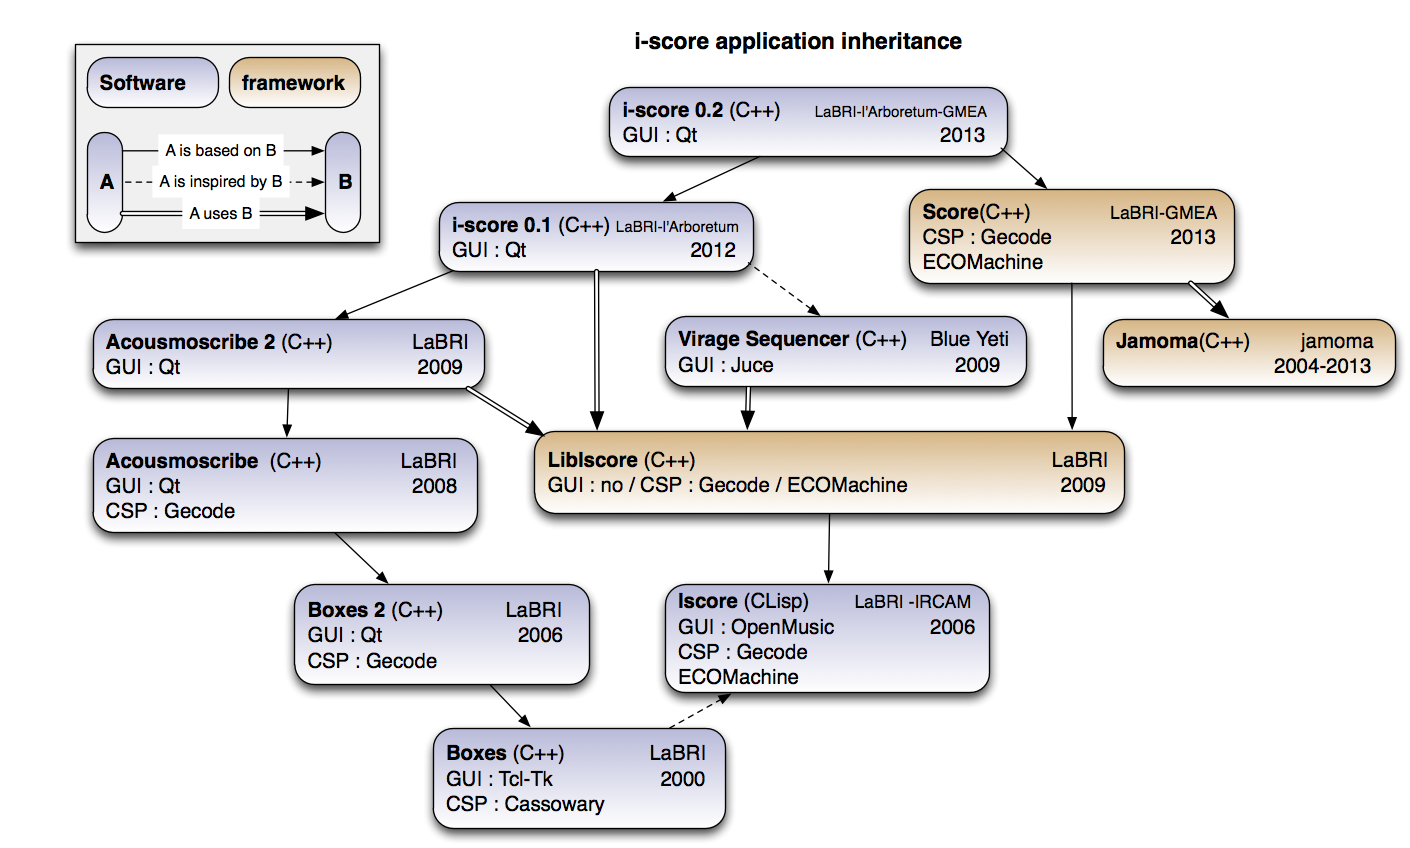
\includegraphics[scale=0.4]{images/iscoreHeritage.png}
	\caption{Les racines du logiciel i-score}
	\label{figheritageIScore}
\end{figure}

Actuellement, il incarne à la fois l'outil permettant d'écrire les scénarios, et de les exécuter.

Deux versions d'i-score (captures d'écran en \cref{figIScore}) sont en développement parallèle : i-score 0.2, une version fonctionnelle mais qui n'inclut pas les travaux les plus récents du paradigme \ac{OSSIA}, et i-score 0.3, une version pour l'instant non-fonctionnelle, mais qui a pour vocation de représenter l'état actuel du développement théorique.

\begin{figure}[H]
	\centering
	\begin{subfigure}{.5\textwidth}
		\centering
		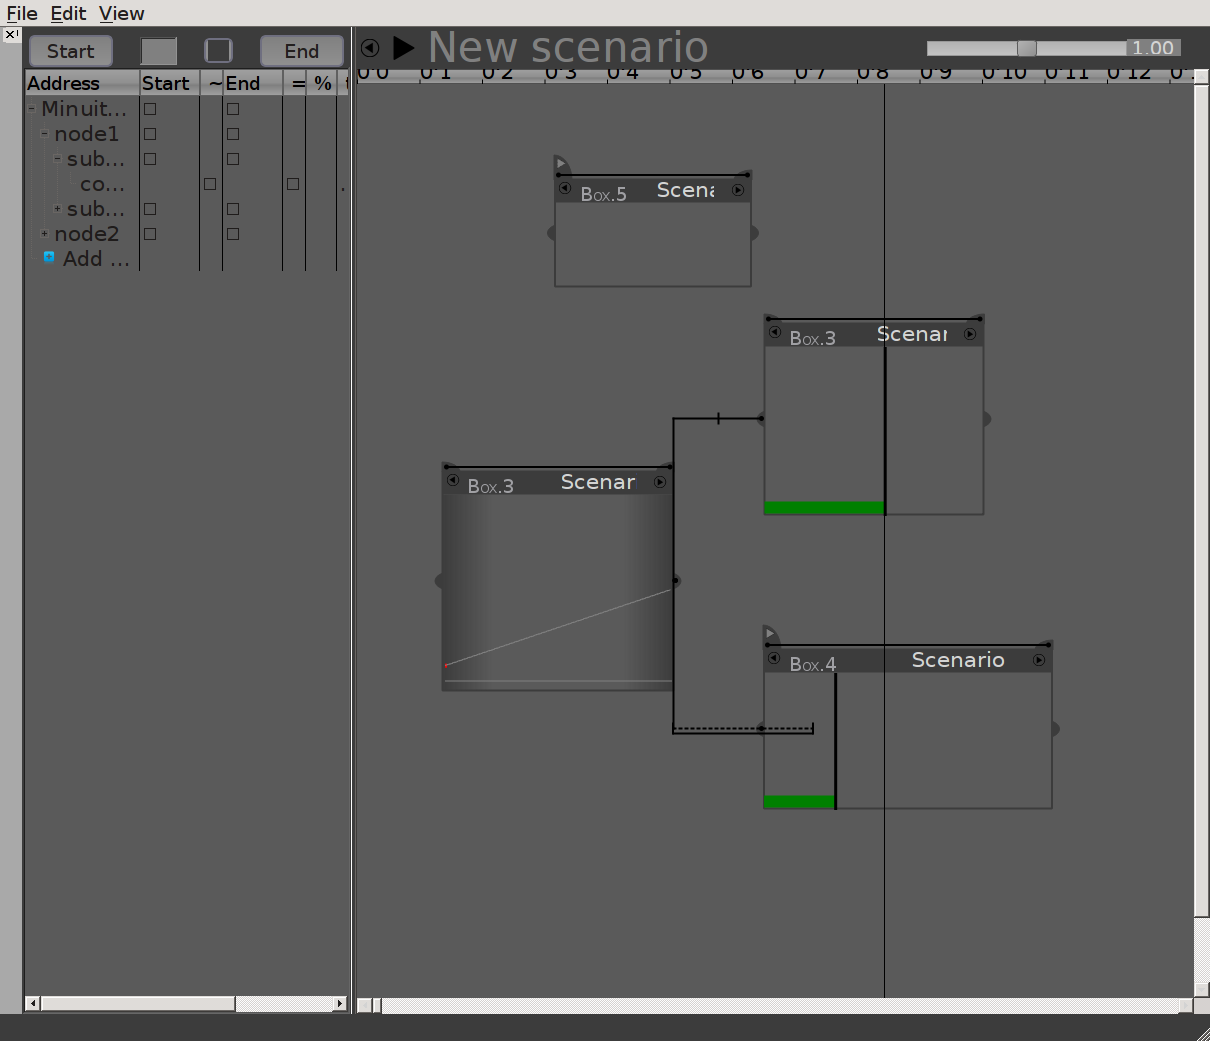
\includegraphics[scale=0.2]{images/iscore02.png}
		\caption{Version 0.2}
	\end{subfigure} 
	
	\vspace{1em}
	
	\begin{subfigure}{.5\textwidth}
		\centering
		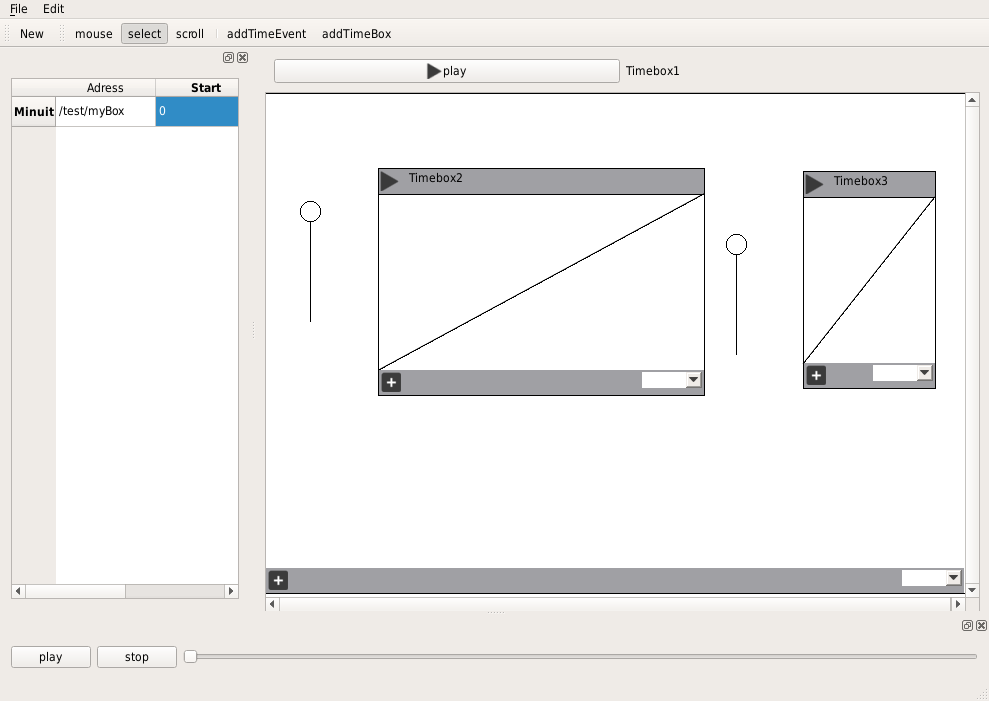
\includegraphics[scale=0.2]{images/iscore03.png}
		\caption{Version 0.3}
	\end{subfigure}
	
	\caption{Captures d'écran des deux version d'i-score.}
	\label{figIScore}
\end{figure}

\subsection{Score et API OSSIA}
\subsubsection{Score}
Score est la bibliothèque sous-jacente qui comporte la logique utilisée pour faire l'exécution d'i-score. Elle contient différents moteurs :

\begin{itemize}
	\item Un moteur d'exécution à base de réseaux de Petri.
	\item Un résolveur de \ac{CSP}, utilisé pour l'édition et plus spécifiquement le déplacement des boîtes.
\end{itemize}

Cette bibliothèque utilise le cadriciel \brand{Jamoma}.

\subsubsection{API}
La version 0.3 d'i-score se base sur une \ac{API}, qui offre toutes les possibilités de gestion de scénario directement au programmeur, de manière à ce que d'autres applications puissent être conçues par dessus. Par exemple, des acteurs du jeu vidéo sont intéressés par le fonctionnement offert par \ac{OSSIA} dans un environnement \brand{Unity}. 

\section{Organisation au cours du stage}
Cette partie précisera le déroulement de mon stage : compréhension du sujet, recherche, implémentation\dots

Pour rappel, le sujet précis du stage était : 
\begin{center}
	\noindent\fbox{\parbox{31em}{Répartition du séquenceur multimedia i-score sur plusieurs machines}}
\end{center}

L'énoncé complet du sujet est disponible en \cref{apx.SujetStage}.
\subsection{Attentes}
\label{sectionAttentes}
Les différents acteurs du projet ont tous eu des attentes différentes par rapport à mon stage.

Néanmoins, il est ressorti des réunions les points suivants : 
\begin{itemize}
	\item La répartition peut être faite au niveau des processus ou des scénarios.
	\item Il est nécessaire de pouvoir grouper facilement les parties censées s'exécuter sur une même machine.
	\item Le backup doit être rendu possible.
	\item Le choix de synchroniser ou non est laissée au compositeur.
	\item Un des intérêts principaux est l'embarqué, que ce soit sur des micro-ordinateurs comme \brand{Raspberry Pi} et \brand{BeagleBoard}, ou bien sur des smartphones et tablettes tactiles.
	\item Le processus de composition doit pouvoir lui aussi être réparti (ou du moins accessible à plusieurs utilisateurs simultanément).
	\item Le formalisme doit être modifié pour prendre en compte la répartition.
	\item L'interface utilisateur doit être modifiée de manière à pouvoir cacher les parties qui s'exécutent à distance.
	\item Une interface utilisateur "chef d'orchestre" doit être présente et permettre de pouvoir tout voir et tout modifier.
\end{itemize}

Au niveau de la répartition, plus précisément, deux possibilités principales ont été vues comme désirables par les compositeurs : 
\begin{itemize}
	\item Le déplacement : le fait de déporter l'exécution d'un processus ou scénario sur une autre machine.
	\item La duplication : le fait de copier l'exécution d'un processus ou scénario sur une autre machine.
\end{itemize}

La duplication peut avoir une arité définie ou indéfinie, c'est à dire que le nombre de machines n'est pas forcément connu à l'avance.

Au niveau plus précis des processus, il a été envisagé de concevoir des cas particuliers permettant notamment de réaliser des opérations sur un groupe de signaux entrants. Par exemple, si onze machines sont lancées, dont une "maître" et dix exécutant un sous-scénario spécifique, on veut que les dix puissent agir chacune indépendamment sur un paramètre donné, et prendre comme résultat la moyenne, la somme, le minimum, le maximum, ou autre, de la valeur de ce paramètre sur les dix machines.

\subsubsection{Exemple dans le formalisme}
Un exemple, présenté en \cref{fig.RepartOSSIA}, a été conçu pour permettre de mettre en valeur les possibilités offertes.

Il est inspiré de l'exemple canonique du moine d'\ac{OSSIA}, présent en \cref{apx.OSSIAExemple}, et suit la même nomenclature.

\begin{figure}[h]
	\centering
	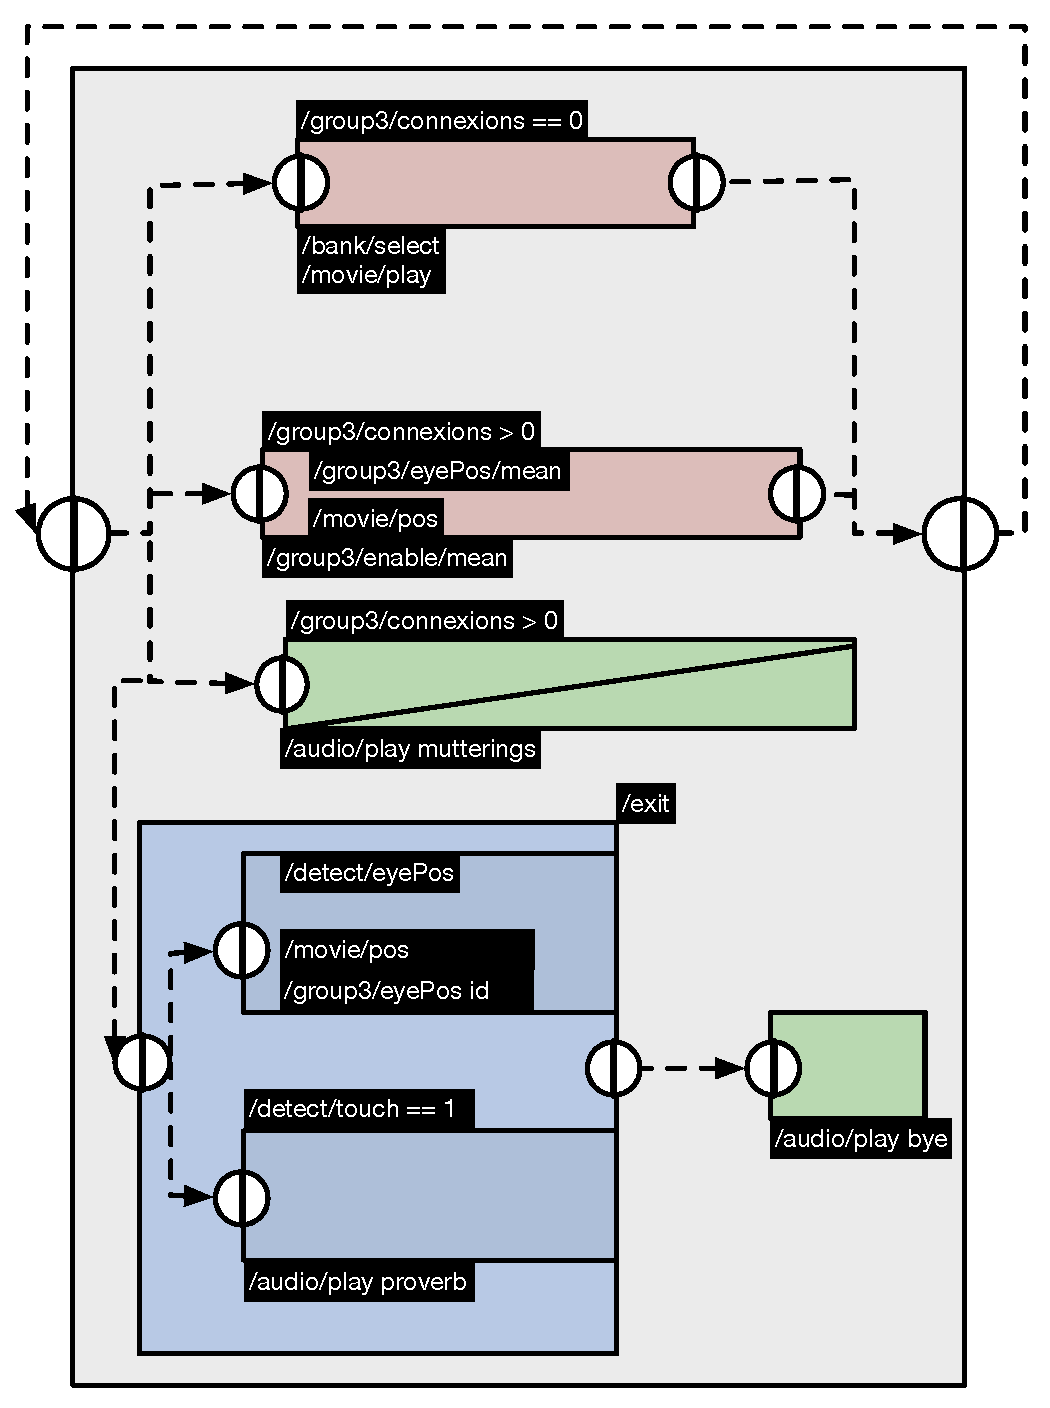
\includegraphics[scale=0.7]{images/ossiaDistri.pdf}
	\caption{Exemple de répartition dans le formalisme \brand{OSSIA}.}
	\label{fig.RepartOSSIA}
\end{figure}

Les couleurs représentent les groupes.
Il y a ici trois groupes : 

\begin{enumerate}
	\item Le premier groupe, \textcolor{BrickRed}{rouge}, sert à projeter de la vidéo sur un écran géant.
	\item Le second groupe, \textcolor{OliveGreen}{vert}, sert à lire des fichiers sons dans une salle.
	\item Le troisième groupe, \textcolor{SteelBlue}{bleu}, est exécuté sur un nombre quelconque d'appareils, comme des tablettes tactiles.  
\end{enumerate}

Le fonctionnement est le suivant : 
\begin{itemize}
	\item Quand personne n'est connecté, des vidéos quelconques sont jouées sur le vidéoprojecteur.
	\item Quand quelqu'un est connecté, il voit sur sa tablette un moine apparaître, qui suit le mouvement de ses yeux.
	\item Quand quelqu'un touche sa tablette, le moine de sa tablette récite un proverbe.
	\item Quand quelqu'un est connecté, un moine s'affiche sur l'écran géant. Le moine regarde dans la direction moyenne des moines présents sur les tablettes connectées au système. Des murmures sont aussi joués par le système de son, avec une augmentation continue et linéaire d'un paramètre (comme volume), puis son retour à zéro.
	\item Quand quelqu'un se déconnecte, un message d'au revoir est dit dans la salle.
\end{itemize}

Les dispositifs suivants sont nécessaires pour exécuter ce scénario : 
\begin{itemize}
	\item Une machine dédiée à l'audio reliée au système de son.
	\item Une machine dédiée à la vidéo reliée au vidéoprojecteur.
	\item Un ensemble de tablettes ou téléphones tactiles avec une caméra en face avant, un logiciel de vidéo, et logiciel d'eye-tracking.
\end{itemize}

Il n'y a pas besoin de machine spécifiquement maîtresse : une des deux machines audio ou vidéo peut en faire office.
Néanmoins, une telle machine peut être rajoutée.
\subsection{Problèmes posés par la répartition}
Un des problèmes majeurs ici est le besoin de synchronisation avec une horloge physique. En effet, les relations entre débuts et fins d'évènements sont données sous forme de millisecondes les séparant, les réseaux étant temporels. Ainsi, les mécanismes d'horloges vectorielles et logiques ne sont pas directement applicables.

Le deuxième problème est qu'il n'est pas réellement question de répartition au sens couramment entendu dans le domaine de l'informatique répartie. En effet, ici, les processus correspondent à des besoins physiquement présents sur des machines et qui ne peuvent pas être déplacés sur d'autres machines. Par exemple, une machine peut avoir une sortie vidéo, et une autre machine une carte son : cela conditionne pour le compositeur l'endroit ou s'exécute un processus, selon qu'il soit relatif à l'image ou au son.

Idéalement, il serait possible de faire une différenciation automatique, néanmoins, deux aspects s'y opposent : 
\begin{itemize}
	\item Le compositeur désire avoir le choix pour la répartition.
	\item Score ne communique qu'avec des messages \ac{OSC}. Un message \ac{OSC} a le format suivant : 
	\begin{verbatim} /adresse/où/écrire argument1 argument2 ... \end{verbatim}.
	
	Les adresses sont laissées à la discrétion des logiciels avec lesquels Score communique, car non standardisées. Il n'est donc pas possible de savoir quel type d'information est communiqué. 
\end{itemize}
Un troisième point, limitant, à tenir en compte, est celui de la gestion de l'interactivité. Dans ce cas, l'impact de la latence due au réseau physique est inévitable, si par exemple un artiste décide d'activer une fonction qui est censée s'exécuter sur une autre machine.


\subsection{Définition du travail à réaliser}
Étant donné la nature duale du stage, mon travail a été séparé en deux parties qui se sont précisées au fil des réunions avec mes encadrants.

\subsubsection{Recherche théorique sur les réseaux de Petri}
Il est apparu assez clairement que la majorité de mon travail théorique porterait sur les réseaux de Petri, car l'intérêt majeur est d'avoir une exécution répartie des scénarios.

J'ai donc essayé de réaliser un existant à jour sur ce sujet, ainsi que sur celui des dernières avancées en répartition et en synchronisation de machines et d'horloges.
Néanmoins, malgré des rencontres avec plusieurs enseignants, je n'ai pas trouvé d'existant portant spécifiquement sur l'exécution des réseaux de Petri dans un cas réparti.
Cette phase est détaillée au \cref{chapterStateOfTheArt}.

Par la suite, j'ai essayé de concevoir des méthodes théoriques pouvant répondre au problème.
J'ai ensuite choisi celle qui a semblé la plus pertinente en les comparant, et ai essayé de prouver sa correction, ainsi que de proposer des améliorations.
Ce travail est présenté dans le \cref{chapterApports}.

\subsubsection{Travail de conception}
La conception a été divisée en trois parties : 
\begin{itemize}
	\item Choix et prise en main des technologies à utiliser et de la position où mon travail doit se situer : i-score 0.2, 0.3, API Score\dots
	\item Conception d'un logiciel de test de répartition de réseaux de Petri.
	\item Intégration des idées présentées en \cref{sectionAttentes} dans i-score.
\end{itemize}

Elle a été suivie d'une phase d'implémentation.

Les détails se trouvent au \cref{chapterImpl}.

\subsubsection{Organisation temporelle}
Je me suis principalement organisé en sprints de 15 jours, qui pouvaient parfois être ponctués par des évènements particuliers. Le détail est présent en \cref{tbl.Timeline}.

\begin{table}[H]
	\centering
	\begin{tabu} to \linewidth {r |@{\vtbullet} X[l]}
		Début à mi-février & Prise en main du sujet \newline \\
		10 et 11 février & Première réunion \ac{OSSIA} \newline \\
		Mi à fin février & Recherche d'existant et portage de \brand{Jamoma} et i-score sous Linux \newline \\
		Début à mi-mars & Conception de l'application de test de répartition, portage sous \brand{Android} et plate-formes \brand{ARM} \newline \\
		14 et 15 mars & Seconde réunion \ac{OSSIA} \newline \\
		Mi-mars & Préparation et rendu du rapport à 6 semaines pour l'ENSEIRB-MATMECA. \newline \\
		20 mars & Présentation à un GT du Scrime \newline \\
		Mi à fin mars &  Essais de conception des algorithmes de répartition de réseaux de Petri \newline \\
		Début à mi-avril & Formalisation et vérification, portage de \brand{Jamoma} sous \gls{CMake} \newline \\
		Mi à fin avril & Conception et implémentation de l'\ac{API} dédiée à la répartition dans Score \newline \\
		Début à mi-mai & Rédaction du présent mémoire \newline \\
		14, 15, 16 Mai & Troisième réunion \ac{OSSIA} \newline \\
		Mi à fin mai & Rédaction du mémoire pour l'ENSEIRB-MATMECA, préparation des soutenances \newline \\
		Début Juin & Continuation de l'implémentation, soutenances \\
	\end{tabu}
	\caption{Organisation au cours du stage}
	\label{tbl.Timeline}
\end{table}